\section{Resultados Obtidos}

A execução dos experimentos em um conjunto de instâncias variadas permitiu uma análise aprofundada do comportamento da heurística de alocação de registradores.
Os testes foram projetados para avaliar o desempenho do algoritmo sob diferentes cenários de pressão de quantidade de usos de cada variável
(variando o limite superior) e a quantidade de variáveis. A seguir, são apresentados e discutidos os resultados quantitativos.

\subsection{Resultados Quantitativos}

Os experimentos foram executados três vezes para cada configuração, e os tempos de execução foram registrados.
A Tabela~\ref{tab:resultados} consolida estes dados, apresentando o tempo médio de execução e o desvio padrão correspondente para
cada classe de teste e tamanho de instância (número de variáveis).

\begin{table}[h!]
\centering
\caption{Tempo médio de execução e desvio padrão para diferentes cenários de teste.}
\label{tab:resultados}
\sisetup{
  table-format=2.6,
  round-mode=places,
  round-precision=6
}
\begin{tabular}{l l l S}
\toprule
\textbf{Tipo de Teste} & {\textbf{Instância}} & {\textbf{Tempo Médio (s)}} & {\textbf{Desvio Padrão (s)}} \\
\midrule
teste-lim-sup-5   & 10   & 0.000135 & 0.000006 \\
                  & 100  & 0.022424 & 0.000096 \\
                  & 200  & 0.095923 & 0.007000 \\
                  & 500  & 0.654350 & 0.004085 \\
                  & 1000 & 3.753158 & 0.081135 \\
\midrule
teste-padrao      & 10   & 0.000135 & 0.000005 \\
                  & 100  & 0.095402 & 0.001427 \\
                  & 200  & 0.573312 & 0.002754 \\
                  & 500  & 3.807789 & 0.014870 \\
                  & 1000 & 21.030808 & 0.207316 \\
\midrule
teste-lim-sup-30  & 10   & 0.000166 & 0.000043 \\
                  & 100  & 0.328989 & 0.011429 \\
                  & 200  & 1.377198 & 0.029020 \\
                  & 500  & 17.993473 & 0.191330 \\
                  & 1000 & 51.772303 & 0.286317 \\
\bottomrule
\end{tabular}
\end{table}

\subsection{Análise dos Resultados}

A análise dos dados apresentados na Tabela~\ref{tab:resultados} revela tendências importantes sobre o comportamento do algoritmo.

\paragraph{Análise de Escalabilidade} Para todos os tipos de teste, observa-se um crescimento consistente no tempo de execução à medida que 
o número de variáveis da instância aumenta. Este crescimento é notavelmente não linear, indicando que a complexidade do problema de coloração
aumenta significativamente com o tamanho do grafo de interferência. Mesmo com a heurística tendo uma complexidade polinomial, o maior impacto no tempo
de execução se dá por causa da reescrita do "programa". Pois isso adiciona uma quantidade imensa de nós para cada reescrita. Para fins de comparação, observou-se
um aumento na quantidade de nós em alguma execuções com inicialmente 1000 variáveis, terminando com cerca de 8000 variáveis, devido ao split das variáveis que seriam
despejadas.


\paragraph{Impacto da quantidade de usos de variáveis (Limite Superior)} A variação no limite superior de usos de variáveis(`k`) apresentou o impacto
mais significativo no desempenho.
\begin{itemize}
    \item \textbf{Cenário Intenso (k=30):} O teste \texttt{teste-lim-sup-30} foi, de longe, o que apresentou os maiores tempos de execução. Com um grande número de usos de cada variável, a liveness analysis gera intervalos cada vez maiores e com cada vez mais interferências. Além disso, quando as variáveis são divididas em variáveis com tempos de vida menor, a quantidade de variáveis aumenta muito, de forma que a próxima iteração do algoritmo com as novas variáveis demore ainda mais.
    \item \textbf{Cenário Restrito (k=5):} Inversamente, o teste \texttt{teste-lim-sup-5} foi o mais rápido. Como existiam menos usos de cada variável, duas coisas importantes acontecem, o liveness dela tende a ser menor, e principalmente, quando ela é dividida em outras variáveis temporárias, a quantidade de variáveis para a próxima execução do algoritmo não aumenta tanto assim, melhorando a eficiência do algoritmo.
    \item \textbf{Cenário Padrão (k=15):} O teste \texttt{teste-padrao}, que representa nosso caso base, situa-se entre os dois extremos, indicando um equilíbrio entre as quantidades de variáveis sendo divididas para as execuções seguintes.
\end{itemize}

\subsection{Visualização Gráfica}

Para melhor ilustrar as tendências de escalabilidade e o impacto dos parâmetros, o Gráfico~\ref{fig:grafico-resultados} plota o
tempo médio de execução em função do número de variáveis da instância para cada tipo de teste. A escala do eixo Y é logarítmica
para acomodar a grande variação nos tempos de execução.

\begin{figure}[ht!]
    \centering
    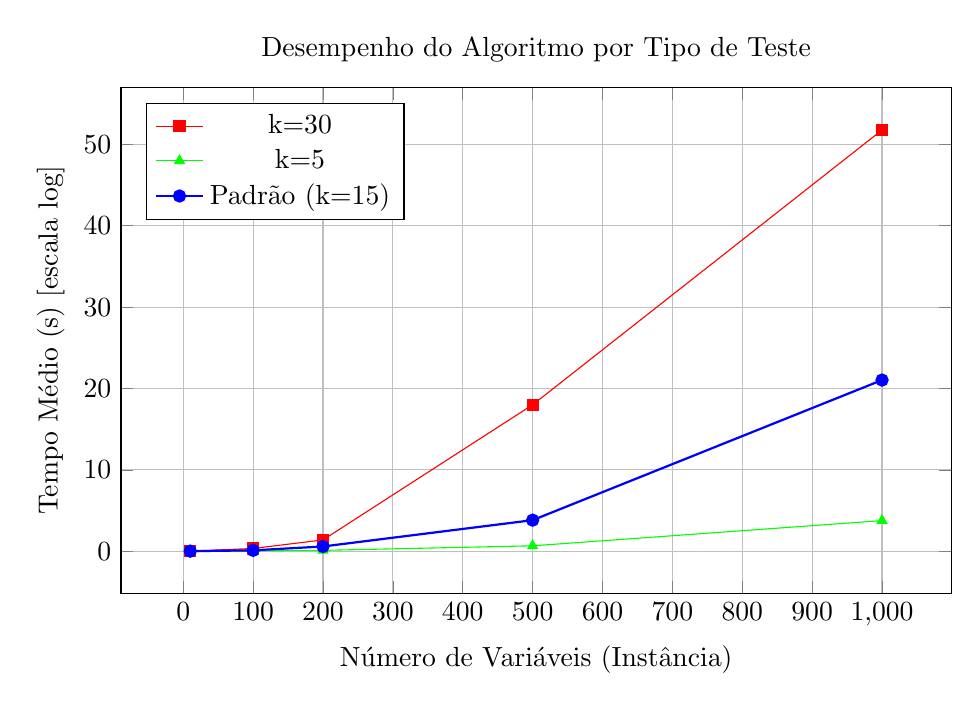
\begin{tikzpicture}
        \begin{axis}[
            title={Desempenho do Algoritmo por Tipo de Teste},
            xlabel={Número de Variáveis (Instância)},
            ylabel={Tempo Médio (s) [escala log]},
            legend pos=north west,
            grid=major,
            width=\textwidth,
            height=8cm,
        ]
        
        \addplot[mark=square*, red] coordinates {(10,0.000166) (100,0.328989) (200,1.377198) (500,17.993473) (1000,51.772303)};
        \addlegendentry{k=30}
        
        \addplot[mark=triangle*, green] coordinates {(10,0.000135) (100,0.022424) (200,0.095923) (500,0.654350) (1000,3.753158)};
        \addlegendentry{k=5}
        
        \addplot[mark=*, thick, blue] coordinates {(10,0.000135) (100,0.095402) (200,0.573312) (500,3.807789) (1000,21.030808)};
        \addlegendentry{Padrão (k=15)}
        
        \end{axis}
    \end{tikzpicture}
    \caption{Comparação do tempo de execução.}
    \label{fig:grafico-resultados}
\end{figure}

O gráfico evidencia claramente o comportamento discutido: a linha correspondente a \texttt{k=30} (vermelha) se destaca com os maiores
tempos, enquanto a linha para \texttt{k=5} (verde) permanece consistentemente como a mais rápida para instâncias maiores. As demais configurações
apresentam um desempenho intermediário e muito próximo entre si.


\subsection{Discussão sobre a Validade das Instâncias}

Uma consideração fundamental para a interpretação dos resultados é a natureza das instâncias geradas pelo simulador. Especificamente, a implementação atual não modela o \textbf{princípio da localidade}, um comportamento prevalente em software real.

No simulador, os usos de uma variável são distribuídos de forma semi-aleatória ao longo de todo o código. Este método pode gerar variáveis com \textit{live ranges} longos e fragmentados, que se estendem por múltiplos escopos. Tal comportamento contrasta com o de programas típicos, onde o tempo de vida de uma variável é frequentemente restrito a uma única função ou a um laço de repetição.

Como consequência, os grafos de interferência gerados, embora válidos, podem apresentar uma topologia menos comum em cenários práticos. Portanto, os resultados obtidos são uma excelente avaliação da robustez da heurística em grafos complexos, mas a sua performance em códigos com alta localidade não foi avaliada devido a limitação da atual implementação do gerador.
